\begin{figure}[htbp]
  \centering
  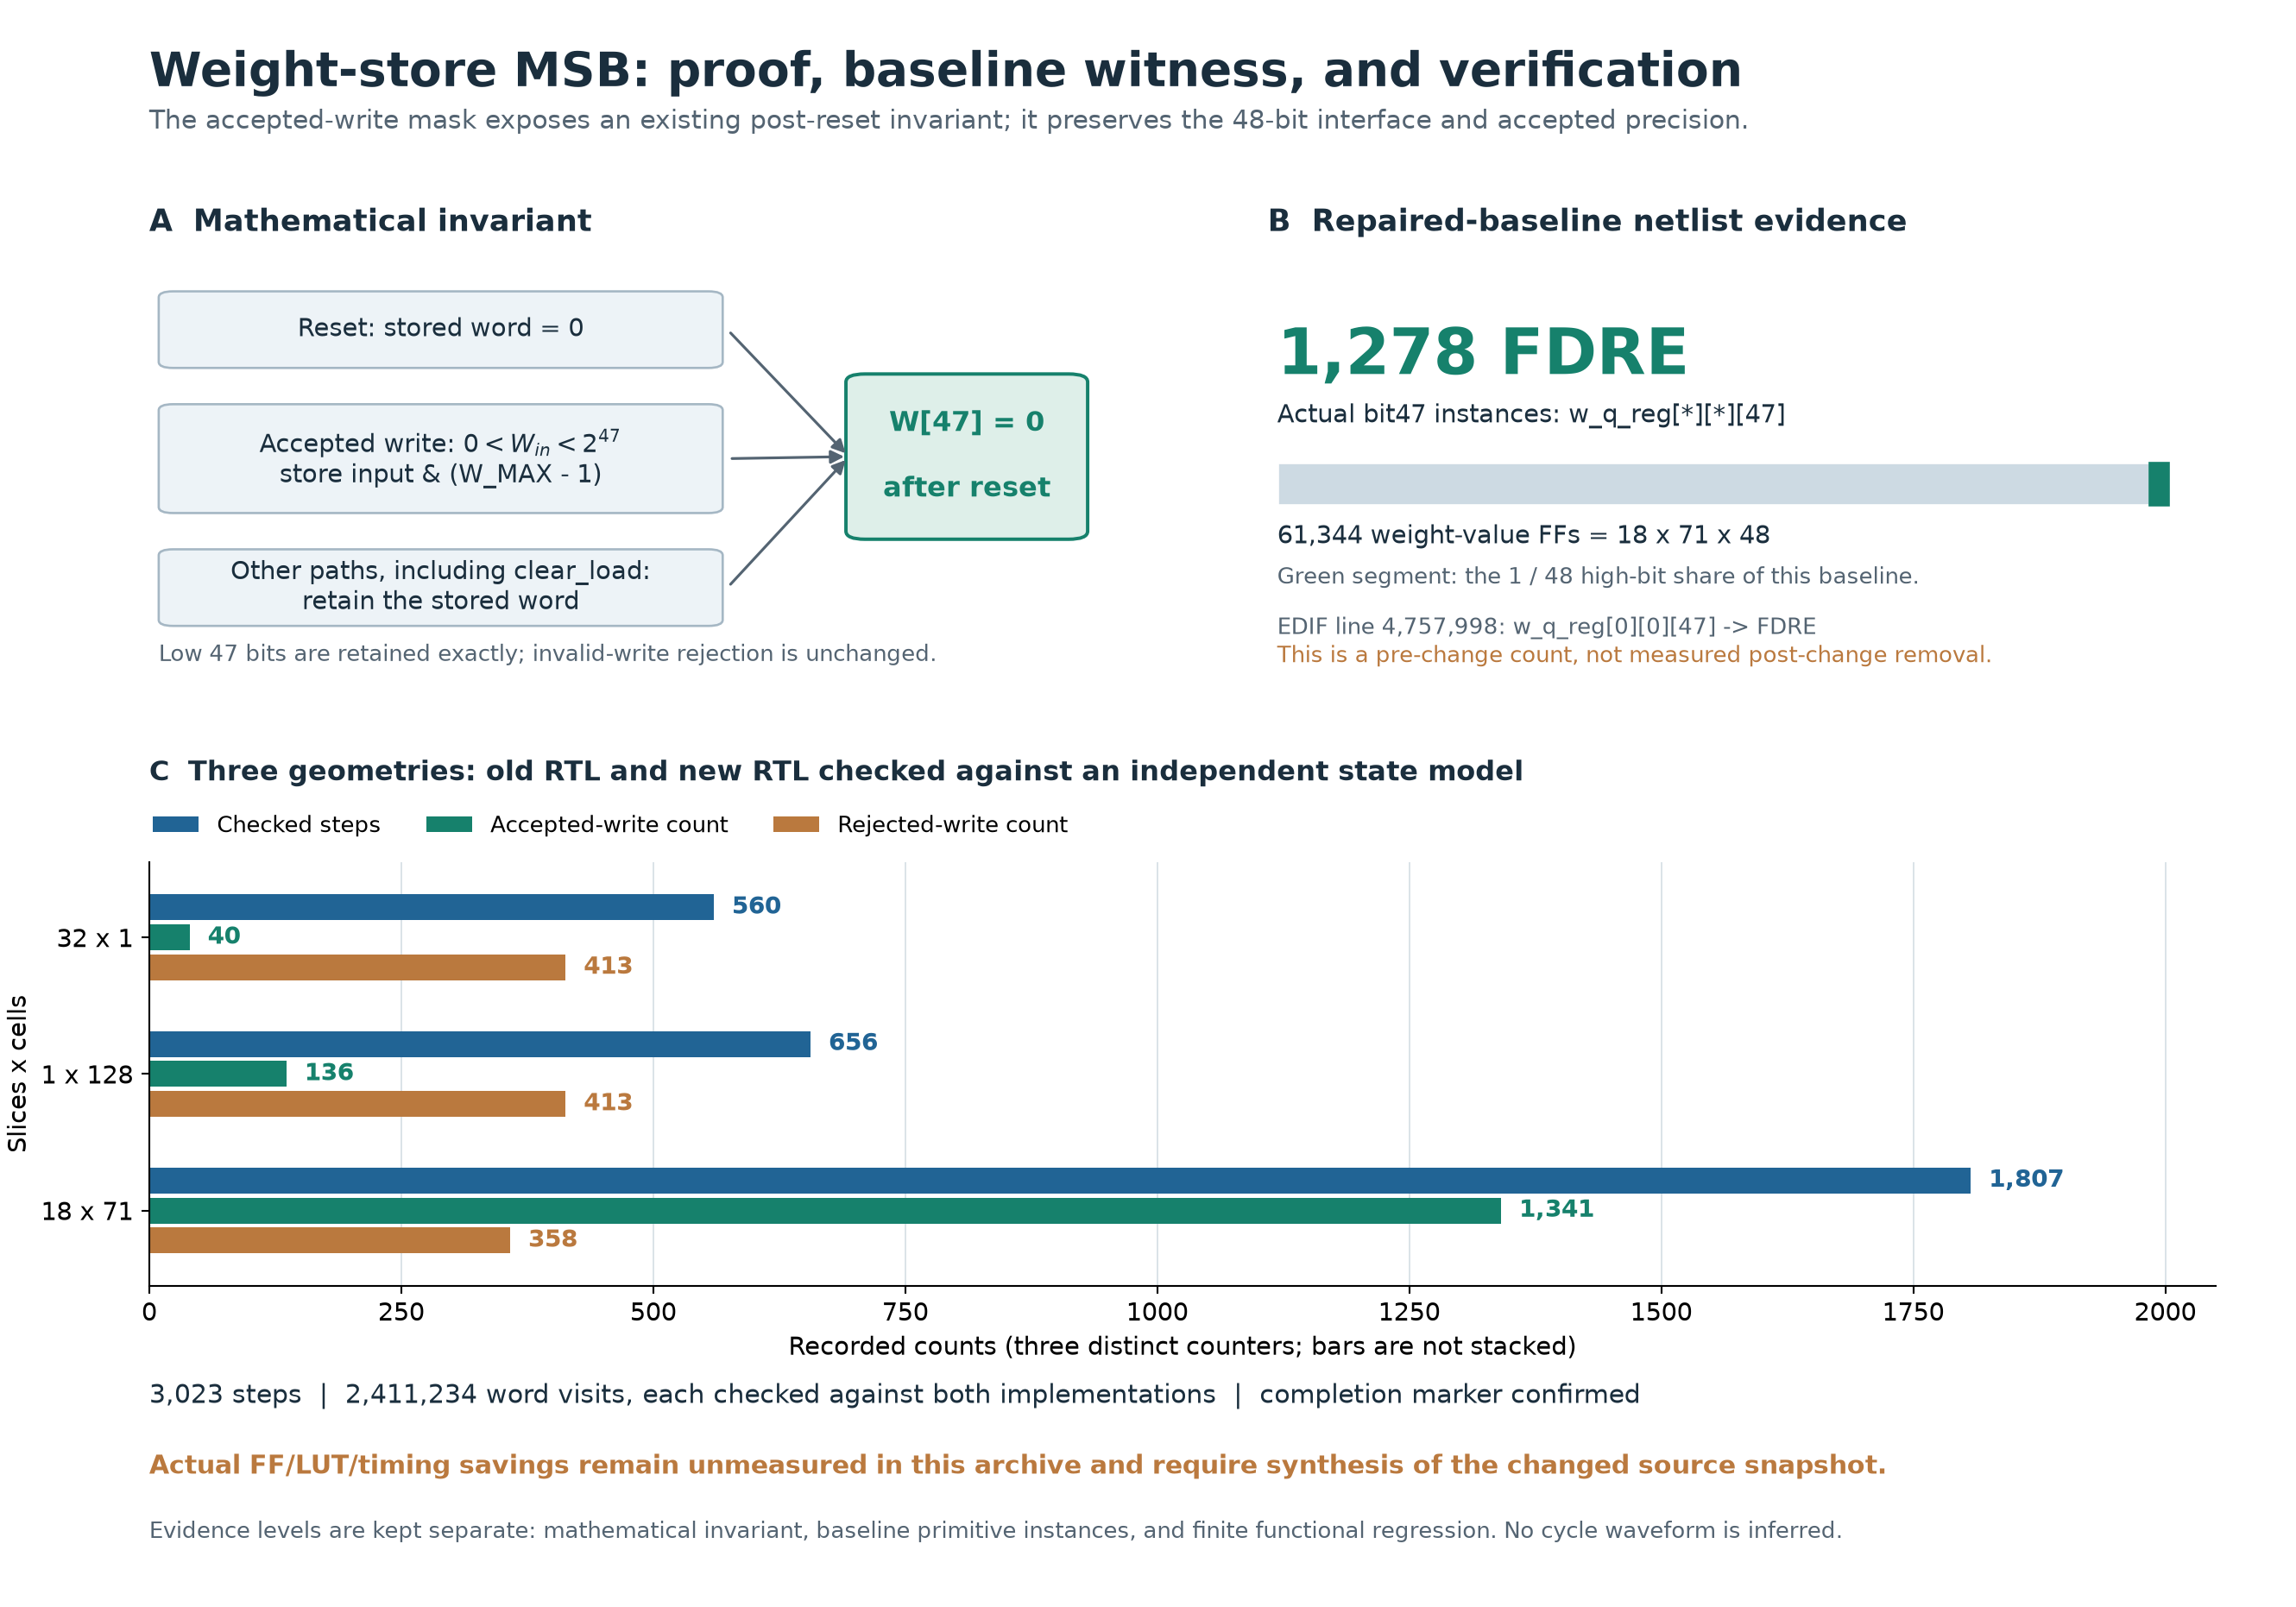
\includegraphics[width=\textwidth]{figures/40_weight_msb_evidence.png}
  \caption{权重存储最高位优化的三层证据。A：复位写零、合法写入满足$0<W<2^{47}$、其他分支保持原值，因而可由归纳法证明复位后的$W[47]=0$；显式写入掩码保留低47位及原有非法写入拒绝行为。B：修复后的基线网表中，61,344个权重数值触发器确实包含1,278个第47位FDRE实例，绿色段仅表示这一基线的$1/48$份额，不能解释为已测得的优化后面积节省。C：三种几何配置的独立状态参考分别检查560、656、1,807步，共3,023步；接受写入、拒绝写入与检查步数是三个不同计数器，图中不堆叠、不相加。按各配置的检查步数乘以存储单元数，共访问2,411,234个权重字，每次均对照修改前、修改后实现；不能再将两种实现的比较次数倍增为覆盖数量。数据来自\code{weight_msb/verification_manifest.json}、\code{equiv.run.log}与\code{vivado_structure/baseline_weight_msb_witness.json}，制图脚本逐项核对归档哈希与完成标记。图中没有重建逐拍波形；修改后真实FF、LUT和时序收益仍需对相应源码快照重新综合测量。}
  \label{fig:weight-msb-evidence}
\end{figure}
